Sharing resources securely across departments or teams in an organisation is a difficult task, with common methods relying on forms of \acrfull{rbac} \citep{Sandhu1996} to grant access to, often unencrypted, resource buckets. This enforces a requirement that users explicitly trust the service they are using and that it is securely designed and implemented properly.

Users must also trust that the access control implemented has been configured correctly to deny access to resources that a user is not authorised for. In practice this is complex to configure, as organisational hierarchies are complex in layout and depth \citep{Dooley2002}.
\vskip 0.5em
Often the level of granularity for access control is too complex for \acrshort{rbac} to enforce and organisations risk accidental access grants through roles that are too expansive in permissions.

These problems can be solved with the use of an \acrfull{abac} \citep{Hu2014} system, utilising a policy language such as \acrshort{xacml} \citep{Parducci2010} to create bespoke, per-resource attribute policies that define specific access restrictions for the resource they are protecting.
\vskip 0.5em
Both \acrshort{rbac} \& \acrshort{abac} systems do not offer data confidentially however, with resources still stored in an unencrypted format. At-rest encryption can be employed to combat this risk, however configuring a bridge between the encryption service and the access control service is difficult and introduces many security pitfalls regarding storage of the decryption keys.

This can all be solved with the use of an \acrfull{abe} system, as described by \citet{Sahai2005} \& \citet{Waters2011}. Which improves security by processing the encryption of resources through a proprietary policy language which allows for \acrshort{abac}-like granular access policies that are \textit{cryptographically} embedded into resources.
\vskip 0.5em
This project developed a complete resource server system, named further as the \theResServer system, which refers to the entire suite of tools developed for the system. The \theResServer system is considered complete as it encompasses all the software required to offer the secure upload \& download of shared resources between a set of users. The \theResServer system is designed such that it is never aware of the contents of any resources uploaded, and implicitly the resources will remain secure even in the event of the system becoming compromised.

\begin{figure}[htp]
  \centering
  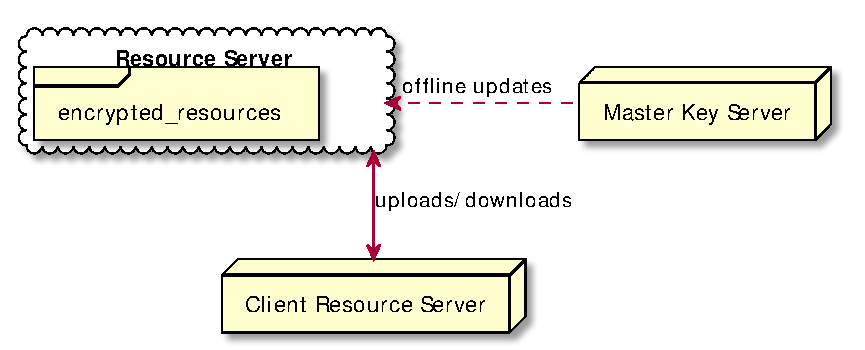
\includegraphics[width=0.7\linewidth,keepaspectratio]{images/infrastructure/deployment_abbrv.pdf}

  \caption{A high-level diagram of the \acrshort{dcs} \theResServer system.}

  \label{fig:deployment_abbrv_diagram}
\end{figure}

\Cref{fig:deployment_abbrv_diagram} represents the \theResServer system at a high level, with two servers: an offline \emph{cold storage} \acrfull{mks} to generate user keys and a separate, online \acrfull{prs} to store and manage the \acrshort{abe} encrypted resources. Additionally, a client tool, the \acrfull{crs}, is also shown communicated with the \acrshort{prs} in order to simplify communication with system for a user, with use of a simple \acrshort{gui}.
